%%%%%%%%%%%%%%%%%%%%%%%%%%%%%%%%%%%%%%%%%%%%%%%%%%%%%%%%%%%%%%%%%%%%%%
%%  Copyright by Wenliang Du.                                       %%
%%  This work is licensed under the Creative Commons                %%
%%  Attribution-NonCommercial-ShareAlike 4.0 International License. %%
%%  To view a copy of this license, visit                           %%
%%  http://creativecommons.org/licenses/by-nc-sa/4.0/.              %%
%%%%%%%%%%%%%%%%%%%%%%%%%%%%%%%%%%%%%%%%%%%%%%%%%%%%%%%%%%%%%%%%%%%%%%

\newcommand{\commonfolder}{../../common-files}
\documentclass[11pt]{article}

\usepackage[most]{tcolorbox}
\usepackage{times}
\usepackage{epsf}
\usepackage{epsfig}
\usepackage{amsmath, alltt, amssymb, xspace}
\usepackage{wrapfig}
\usepackage{fancyhdr}
\usepackage{url}
\usepackage{verbatim}
\usepackage{fancyvrb}
\usepackage{adjustbox}
\usepackage{listings}
\usepackage{color}
\usepackage{subfigure}
\usepackage{cite}
\usepackage{sidecap}
\usepackage{pifont}
\usepackage{mdframed}
\usepackage{textcomp}
\usepackage{enumitem}


% Horizontal alignment
\topmargin      -0.50in  % distance to headers
\oddsidemargin  0.0in
\evensidemargin 0.0in
\textwidth      6.5in
\textheight     8.9in 

\newcommand{\todo}[1]{
\vspace{0.1in}
\fbox{\parbox{6in}{TODO: #1}}
\vspace{0.1in}
}


\newcommand{\unix}{{\tt Unix}\xspace}
\newcommand{\linux}{{\tt Linux}\xspace}
\newcommand{\minix}{{\tt Minix}\xspace}
\newcommand{\ubuntu}{{\tt Ubuntu}\xspace}
\newcommand{\setuid}{{\tt Set-UID}\xspace}
\newcommand{\openssl} {\texttt{openssl}}


\pagestyle{fancy}
\lhead{\bfseries SEED Labs}
\chead{}
\rhead{\small \thepage}
\lfoot{}
\cfoot{}
\rfoot{}


\definecolor{dkgreen}{rgb}{0,0.6,0}
\definecolor{gray}{rgb}{0.5,0.5,0.5}
\definecolor{mauve}{rgb}{0.58,0,0.82}
\definecolor{lightgray}{gray}{0.90}


\lstset{%
  frame=none,
  language=,
  backgroundcolor=\color{lightgray},
  aboveskip=3mm,
  belowskip=3mm,
  showstringspaces=false,
%  columns=flexible,
  basicstyle={\small\ttfamily},
  numbers=none,
  numberstyle=\tiny\color{gray},
  keywordstyle=\color{blue},
  commentstyle=\color{dkgreen},
  stringstyle=\color{mauve},
  breaklines=true,
  breakatwhitespace=true,
  tabsize=3,
  columns=fullflexible,
  keepspaces=true,
  escapeinside={(*@}{@*)}
}

\newcommand{\newnote}[1]{
\vspace{0.1in}
\noindent
\fbox{\parbox{1.0\textwidth}{\textbf{Note:} #1}}
%\vspace{0.1in}
}


%% Submission
\newcommand{\seedsubmission}{You need to submit a detailed lab report, with screenshots,
to describe what you have done and what you have observed.
You also need to provide explanation
to the observations that are interesting or surprising.
Please also list the important code snippets followed by
explanation. Simply attaching code without any explanation will not
receive credits.}

%% Book
\newcommand{\seedbook}{\textit{Computer \& Internet Security: A Hands-on Approach}, 2nd
Edition, by Wenliang Du. See details at \url{https://www.handsonsecurity.net}.}

%% Videos
\newcommand{\seedisvideo}{\textit{Internet Security: A Hands-on Approach},
by Wenliang Du. See details at \url{https://www.handsonsecurity.net/video.html}.}

\newcommand{\seedcsvideo}{\textit{Computer Security: A Hands-on Approach},
by Wenliang Du. See details at \url{https://www.handsonsecurity.net/video.html}.}

%% Lab Environment
\newcommand{\seedenvironment}{This lab has been tested on our pre-built
Ubuntu 16.04 VM, which can be downloaded from the SEED website. }

\newcommand{\seedenvironmentA}{This lab has been tested on our pre-built
Ubuntu 16.04 VM, which can be downloaded from the SEED website. }

\newcommand{\seedenvironmentB}{This lab has been tested on our pre-built
Ubuntu 20.04 VM, which can be downloaded from the SEED website. }

\newcommand{\seedenvironmentAB}{This lab has been tested on our pre-built
Ubuntu 16.04 and 20.04 VMs, which can be downloaded from the SEED website. }

\newcommand{\nodependency}{Since we use containers to set up the lab environment, 
this lab does not depend too much on our SEED VM. You can do this lab
using other VMs or physical machines. }







\newcommand{\seedlabcopyright}[1]{
\vspace{0.1in}
\fbox{\parbox{6in}{\small Copyright \copyright\ {#1}\ \ by Wenliang Du.\\
      This work is licensed under a Creative Commons
      Attribution-NonCommercial-ShareAlike 4.0 International License.
      If you remix, transform, or build upon the material, 
      this copyright notice must be left intact, or reproduced in a way that is reasonable to
      the medium in which the work is being re-published.}}
\vspace{0.1in}
}






\newcommand{\telnet} {\texttt{telnet}\xspace}
\newcommand{\iptables}{\texttt{iptables}\xspace}
\newcommand{\netfilter}{\texttt{netfilter}\xspace}
\newcommand{\Netfilter}{\texttt{Netfilter}\xspace}

\newcommand{\firewallFigs}{./Figs}
\lhead{\bfseries SEED Labs -- Firewall Lab}

\begin{document}



\begin{center}
{\LARGE Firewall Lab}
\end{center}

\seedlabcopyright{2006 - 2020}



% *******************************************
% SECTION
% ******************************************* 
\section{Overview}

The learning objective of this lab is two-fold: learning
how firewalls work, and setting up a simple firewall
for a network. Students will first 
implement a simple stateless packet-filtering firewall, 
which inspects packets, and decides 
whether to drop or forward a packet based on firewall rules. 
Through this implementation task, students can get the 
basic ideas on how firewall works.


Actually, Linux already has a built-in firewall, also based on 
\texttt{netfilter}. This firewall is called \iptables. 
Students will be given a simple network topology, and are asked to
use \iptables to set up firewall rules to protect the network. 
Students will also be exposed to several other interesting 
applications of \iptables. 
This lab covers the following topics:


\begin{itemize}[noitemsep]
\item Firewall
\item Netfilter
\item Loadable kernel module
\item Using \iptables to set up firewall rules
\item Various applications of \iptables
\end{itemize}


\paragraph{Readings and videos.}
Detailed coverage of firewalls can be found in the following:

\begin{itemize}
\item Chapter 17 of the SEED Book, \seedbook
\item Section 9 of the SEED Lecture, \seedisvideo
\end{itemize}


\paragraph{Lab environment.} \seedenvironmentB




% *******************************************
% SECTION
% ******************************************* 
\section{Environment Setup Using Containers}


In this lab, we need to use multiple machines. 
Their setup is depicted in Figure~\ref{fig:labsetup}.  
We will use containers to set up this lab environment.


\begin{figure}[htb]
\begin{center}
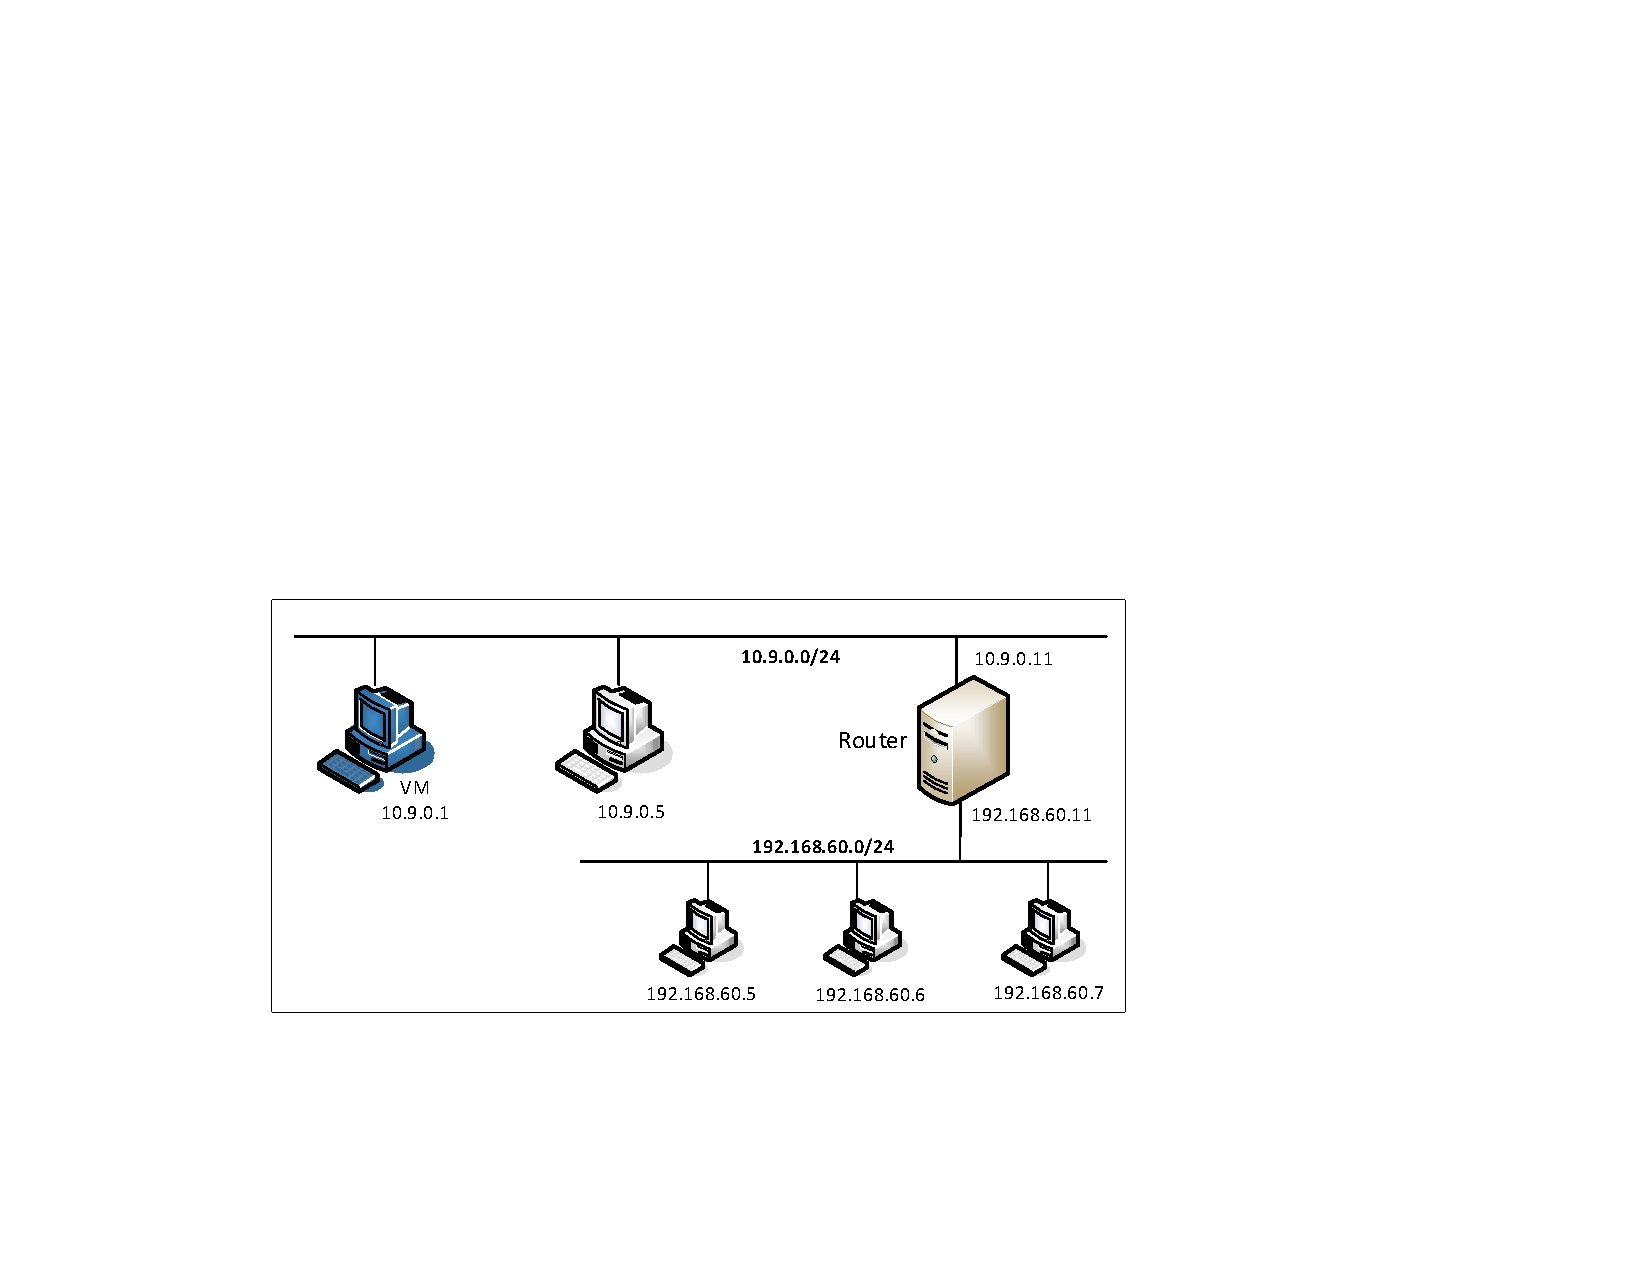
\includegraphics[width=0.8\textwidth]{./Figs/TwoLANs.pdf}
\end{center}
\caption{Lab setup}
\label{fig:labsetup}
\end{figure}


% -------------------------------------------
% SUBSECTION
% -------------------------------------------
\subsection{Container Setup and Commands}
%%%%%%%%%%%%%%%%%%%%%%%%%%%%%%%%%%%%%%%%%%%%
Please download the
\texttt{Labsetup.zip} file to your VM from the lab's website,
unzip it, enter the \texttt{Labsetup} folder, and 
use the \texttt{docker-compose.yml} file to 
set up the lab environment. Detailed explanation
of the content in this file and all the involved 
\texttt{Dockerfile} can be found from the 
user manual, which is linked to the website of this lab.
If this is the first time you set up a SEED lab environment
using containers, it is very important that you read 
the user manual. 

In the following, we list some of the commonly
used commands related to Docker and Compose. 
Since we are going to use 
these commands very frequently, we have created aliases for them
in the \texttt{.bashrc} file (in our provided SEEDUbuntu 20.04 VM).


\begin{lstlisting}
$ docker-compose build  # Build the container image
$ docker-compose up     # Start the container
$ docker-compose down   # Shut down the container

// Aliases for the Compose commands above
$ dcbuild       # Alias for: docker-compose build
$ dcup          # Alias for: docker-compose up
$ dcdown        # Alias for: docker-compose down
\end{lstlisting}


All the containers will be running in the background. To run
commands on a container, we often need to get a shell on
that container. We first need to use the \texttt{"docker ps"}  
command to find out the ID of the container, and then
use \texttt{"docker exec"} to start a shell on that 
container. We have created aliases for them in
the \texttt{.bashrc} file.

\begin{lstlisting}
$ dockps        # Alias for: docker ps --format "{{.ID}}  {{.Names}}" 
$ docksh <id>   # Alias for: docker exec -it <id> /bin/bash

# The following example shows how to get a shell inside hostC
$ dockps
b1004832e275  hostA-10.9.0.5
0af4ea7a3e2e  hostB-10.9.0.6
9652715c8e0a  hostC-10.9.0.7

$ docksh 96
root@9652715c8e0a:/#  

# Note: If a docker command requires a container ID, you do not need to 
#       type the entire ID string. Typing the first few characters will 
#       be sufficient, as long as they are unique among all the containers. 
\end{lstlisting}


If you encounter problems when setting up the lab environment, 
please read the ``Common Problems'' section of the manual
for potential solutions.


%%%%%%%%%%%%%%%%%%%%%%%%%%%%%%%%%%%%%%%%%%%%



% -------------------------------------------
% SUBSECTION
% -------------------------------------------
\subsection{Detach the VM from \texttt{192.168.60.0/24} Network} 
%%%%%%%%%%%%%%%%%%%%%%%%%%%%%%%%%%%%%%%%%%%%

%\paragraph{Removing the Host VM from \texttt{192.168.60.0/24} network.}
When Docker creates a network, it automatically attach the
host machine (i.e., the VM) to the network. In this
case, the host machine is attached to both
networks, and is given the IP address \texttt{10.9.0.1} and
\texttt{192.168.60.1}.
This may create undesirable situations,
so let's remove it.

In our setup, we only want the VM to be connected to
\texttt{10.9.0.0/24}, not to both.
We need to detach the VM from the other network. We cannot simply power down
the interface, because that will affects all the containers on that network.
Our solution is to remove the IP address
of the interface, and then set the routing accordingly. 


\begin{lstlisting}
// Get the name of the interface 
$ ip addr

// Remove the IP address from the interface
$ sudo ip addr flush <interface-name>

// Use 10.9.0.11 as the router to access 192.168.60.0/24
$ sudo ip route add 192.168.60.0/24 via 10.9.0.11
\end{lstlisting}


%%%%%%%%%%%%%%%%%%%%%%%%%%%%%%%%%%%%%%%%%%%%



% *******************************************
% SECTION
% ******************************************* 
\section{Task 1: Implementing a Simple Firewall} 


In this task, we will implement a simple packet filtering 
type of firewall, which 
inspects each incoming and outgoing packets, and enforces the firewall policies 
set by the administrator. Since the packet 
processing is done within the kernel, the filtering must also be 
done within the kernel. Therefore, it seems that implementing such
a firewall requires us to modify the \linux kernel. In the past, 
this had to be done by modifying and rebuilding 
the kernel. The modern \linux 
operating systems provide several new mechanisms 
to facilitate the manipulation of packets without rebuilding
the kernel image. These two mechanisms are 
\textit{Loadable Kernel Module} (\texttt{LKM}) and \texttt{Netfilter}.



% -------------------------------------------
% SUBSECTION
% ------------------------------------------- 
\subsection{Task 1.a: Implement a Simple Kernel Module}


{\tt LKM} allows us to add a new module to the kernel at the runtime. 
This new module enables us to extend the functionalities of the kernel,
without rebuilding the kernel or even rebooting the computer. 
The packet filtering part of a firewall can be implemented as an LKM. 
In this task, we will get familiar with LKM.


The following is a simple loadable kernel module. It prints out 
\texttt{"Hello World!"} when the module is loaded; when the module
is removed from the kernel, it prints out \texttt{"Bye-bye World!"}.
The messages are not printed out on the screen; they are 
actually printed into the \texttt{/var/log/syslog} file. You can
use \texttt{"dmesg | tail -10"} to read the last 10 lines of 
the messages. 


\begin{lstlisting}
#include <linux/module.h>
#include <linux/kernel.h>

int init_module(void)
{
    printk(KERN_INFO "Hello World!\n");
    return 0;
}

void cleanup_module(void)
{
    printk(KERN_INFO "Bye-bye World!.\n");
}
\end{lstlisting}

We now need to create {\tt Makefile}, which includes the following
contents (the above program is named {\tt hello.c}). Then 
just type {\tt make}, and the above program will be compiled
into a loadable kernel module (when you copy and paste the following
into \texttt{Makefile}, make sure replace the spaces before the 
\texttt{make} commands with a tab).


\begin{lstlisting}
obj-m += hello.o

all:
        make -C /lib/modules/$(shell uname -r)/build M=$(PWD) modules

clean:
        make -C /lib/modules/$(shell uname -r)/build M=$(PWD) clean
\end{lstlisting}


Once the module is built by typing {\tt make}, you can use the following commands to 
load the module, list all modules, and remove the module. 
Also, you can use {\tt modinfo mymod.ko} to show information about a 
Linux Kernel module.

\begin{lstlisting}
$ sudo insmod mymod.ko        (inserting a module)
$ lsmod                       (list all modules)
$ sudo rmmod mymod.ko         (remove the module)
$ dmesg | tail -10            (check the messages)
\end{lstlisting}


\paragraph{Task.} Please compile and run this simple kernel module on 
your VM and show your running results in the lab report. 
It should be noted that all the tasks in Task 1 should be 
performed on the VM, but students who are familiar with Docker
are encouraged to deploy the firewall developed in this task
to the router container. 


% -------------------------------------------
% SUBSECTION
% ------------------------------------------- 
\subsection{Task 1.b: Implement a Simple Firewall Using \texttt{Netfilter}}  


In this task, we will write our packet filtering program
as an LKM, and then insert in into the packet processing path
inside the kernel. This cannot be easily done in the past before 
the \Netfilter was introduced into the \linux.

{\tt Netfilter} is designed to facilitate the manipulation of 
packets by authorized users. {\tt Netfilter} achieves this 
goal by implementing a number of {\em hooks} in the 
\linux kernel. These hooks are inserted into various places, 
including the packet incoming and outgoing paths. 
If we want to manipulate the incoming packets, we simply
need to connect our own programs (within LKM) to the 
corresponding hooks. Once an incoming packet arrives, 
our program will be invoked. Our program can decide 
whether this packet should be blocked or not; moreover,
we can also modify the packets in the program.


In this task, you need to use LKM and {\tt Netfilter} to implement
the packet filtering module.  This module will fetch 
the firewall policies from a data structure, and use the 
policies to decide whether packets should be blocked or not.
To make your life easier, so you can focus on the filtering part, 
the core of firewalls, we allow you to hardcode your firewall policies 
in the program. You should support at least three different 
rules. Guidelines on how to use \texttt{Netfilter} can be 
found in Chapter 17 of the SEED book.


Using {\tt Netfilter} is quite straightforward. All we need to do
is to hook our functions (in the kernel module) to the corresponding
{\tt Netfilter} hooks. Here we show an example (the code is in
\path{Labsetup/packet_filter}):


\begin{lstlisting}
#include <linux/module.h>
#include <linux/kernel.h>
#include <linux/netfilter.h>
#include <linux/netfilter_ipv4.h>
#include <linux/ip.h>
#include <linux/tcp.h>


/* This is the structure we shall use to register our function */
static struct nf_hook_ops nfho;

/* This is the hook function itself */
unsigned int hook_func(void *priv, struct sk_buff *skb, 
                       const struct nf_hook_state *state)

{
    /* This is where you can inspect the packet contained in
       the structure pointed by skb, and decide whether to accept 
       or drop it. You can even modify the packet */
 
    struct iphdr *iph;
    struct tcphdr *tcph;
    
    iph = ip_hdr(skb);
    tcph = (void *)iph+iph->ihl*4;
 
    if (iph->protocol == IPPROTO_TCP && tcph->dest == htons(23)) {
      printk(KERN_INFO "Dropping telnet packet to %d.%d.%d.%d\n",
          ((unsigned char *)&iph->daddr)[0],
          ((unsigned char *)&iph->daddr)[1],
          ((unsigned char *)&iph->daddr)[2],
          ((unsigned char *)&iph->daddr)[3]);
      return NF_DROP;       /* Drop this packet */
    } else {
      return NF_ACCEPT;     /* Accept this packet */
    }
}

/* Initialization routine */
int init_module()
{   /* Fill in our hook structure */
    nfho.hook = hook_func;               // Handler function 
    nfho.hooknum  = NF_INET_PRE_ROUTING; // The hook 
    nfho.pf       = PF_INET;
    nfho.priority = NF_IP_PRI_FIRST;     // Make our function first 

    // nf_register_hook(&nfho);               // For Ubuntu 16.04 VM
    nf_register_net_hook(&init_net, &nfho);   // For Ubuntu 20.04 VM
    return 0;
}

/* Cleanup routine */
void cleanup_module()
{
    // nf_unregister_hook(&nfho);             // For Ubuntu 16.04 VM
    nf_unregister_net_hook(&init_net, &nfho); // For Ubuntu 20.04 VM
}
\end{lstlisting}


\paragraph{Note for Ubuntu 20.04 VM:}
The code in the SEED book was developed in Ubuntu 16.04. It needs to be changed slightly 
to work in Ubuntu 20.04. The change is in the hook registration and 
unregistration APIs. See the difference in the following:


\begin{lstlisting}
// Hook registration:
  nf_register_hook(&nfho);                  // For Ubuntu 16.04 VM
  nf_register_net_hook(&init_net, &nfho);   // For Ubuntu 20.04 VM


// Hook unregistration:
  nf_unregister_hook(&nfho);                // For Ubuntu 16.04 VM
  nf_unregister_net_hook(&init_net, &nfho); // For Ubuntu 20.04 VM
\end{lstlisting}
 

\paragraph{Tasks.} Based on the code provided above (they can be downloaded
from the lab's website), please do the following tasks:

\begin{itemize}
\item Compile and run the provided code. Based on your execution results,
explain the purpose of the firewall.  

\item The following are \netfilter hooks. Please replace the 
hook used in the sample code with the ones marked by \ding{81}
and describe your observation.

\begin{lstlisting}
NF_INET_PRE_ROUTING 
NF_INET_LOCAL_IN         (*@\ding{81}@*)
NF_INET_FORWARD 
NF_INET_LOCAL_OUT 
NF_INET_POST_ROUTING     (*@\ding{81}@*)
\end{lstlisting}
\end{itemize}
 



% *******************************************
% SECTION
% ******************************************* 
\section{Task 2: Setting Up a Stateless Firewall}

In the previous task, we had a chance to build a simple firewall using \netfilter. Actually,
\linux already has a built-in firewall, also based on \netfilter. This firewall is called
\iptables. Technically, the kernel part implementation of the firewall
is called \texttt{Xtables}, while \iptables is a user-space program to
configure the firewall. However, \iptables is often used to refer to both the kernel-part
implementation and the user-space program. 



% -------------------------------------------
% SUBSECTION
% ------------------------------------------- 
\subsection{Background of \iptables}

In this task, we will use \iptables to set up a firewall. 
The \iptables firewall is designed not only to filter packets, but also to make changes to
packets. To help manage these firewall rules for different purposes, \iptables organizes all
rules using a hierarchical structure: table, chain, and rules.
There are several tables, each specifying the main purpose of the rules as shown
in Table~\ref{firewall:table:iptables}.
For example, rules for packet filtering should be
placed in the \texttt{filter} table, while rules for making changes to packets should be placed
in the \texttt{nat} or \texttt{mangle} tables.

Each table contains several chains, each of which corresponds to a \netfilter hook. Basically,
each chain indicates where its rules are enforced. For example, rules on
the \texttt{FORWARD} chain are enforced at the \texttt{NF\_INET\_FORWARD} hook, and rules on
the \texttt{INPUT} chain are enforced at the  \texttt{NF\_INET\_LOCAL\_IN} hook.

Each chain contains a set of firewall rules that will be enforced.
When we set up firewalls, we add rules to these chains.
For example, if we would like to block all incoming \telnet traffic, we would
add a rule to the \texttt{INPUT} chain of the \texttt{filter} table.  If we
would like to redirect all incoming \telnet traffic to a different
port on a different host, basically doing port forwarding, we can add a rule to the
\texttt{INPUT} chain of the \texttt{mangle} table, as we need to make changes to packets.


\begin{table}[htb]
        \centering
%       \renewcommand{\arraystretch}{1.2}
        \caption{\iptables Tables and Chains}
        \label{firewall:table:iptables}
        \centering

        \begin{tabular}{|l|l|l|}
                \hline
                \bfseries Table & \bfseries Chain & \bfseries Functionality \\
                \hline\hline
                filter          &    \texttt{INPUT}      & Packet filtering \\
                                &    \texttt{FORWARD}    & \\
                                &    \texttt{OUTPUT}      & \\
                \hline
                nat             &   \texttt{PREROUTING}    & Modifying source or destination \\
                                &   \texttt{INPUT}      & network addresses \\
                                &   \texttt{OUTPUT}      & \\
                                &   \texttt{POSTROUTING}   & \\
                \hline
                mangle          &   \texttt{PREROUTING}    & Packet content modification \\
                                &   \texttt{INPUT}      & \\
                                &   \texttt{FORWARD}     & \\
                                &   \texttt{OUTPUT}      & \\
                                &   \texttt{POSTROUTING}   & \\
                \hline
        \end{tabular}
\end{table}


% -------------------------------------------
% SUBSECTION
% ------------------------------------------- 
\subsection{Using \iptables}


To add rules to the chains in each table, we use the \iptables command,
which is a quite powerful command. 
Students can find the manual of \iptables by typing \texttt{"man iptables"} 
or easily find many tutorials from online. 
What makes \iptables complicated is the many command-line arguments 
that we need to provide when
using the command. However, 
if we understand the structure of these command-line arguments, 
we will find out that the command is not that complicated. 


In a typical \iptables command, we add a rule to or remove a rule 
from one of the chains in one of the tables, so we need to 
specify a table name (the default is \texttt{filter}), a chain name, 
and an operation on the chain. After that, we specify the rule, which
is basically a pattern that will be matched with each of the 
packets passing through. If there is a match, an action will be 
performed on this packet. 
The general structure of the command is depicted in the following:

\begin{lstlisting}
# iptables -t <table> -<operation> <chain>  <rule>   -j <target>
           ---------- --------------------  -------  -----------
              Table          Chain           Rule      Action
\end{lstlisting}


The rule is the most complicated part of the \iptables command. 
We will provide additional information later on when we use 
specific rules. In the following, we list some commonly 
used commands: 


\begin{lstlisting}
// List all the rules in a table (without line number)
$ sudo iptables -t nat -L

// List all the rules in a table (with line number)
$ sudo iptables -t filter -L --line-numbers

// Delete rule No. 2 in the INPUT chain of the filter table 
$ sudo iptables -t filter -D INPUT 2

// Drop all the incoming packets that satisfy the <rule>
$ sudo iptables -t filter -A INPUT <rule>  -j DROP
\end{lstlisting}


\paragraph{Note.} Docker relies on \iptables to manage 
the networks it creates, so it adds many rules to \iptables.
When we manipulate \iptables rules, we should be careful 
not to remove Docker rules. For example, it will be quite
dangerous to run the \texttt{"iptables -F"} command, because 
it removes all the rules in the \texttt{filter} table,
including many of the Docker rules. That will cause 
trouble to Docker containers. 


% -------------------------------------------
% SUBSECTION
% ------------------------------------------- 
\subsection{Set Up a Stateless Firewall}

In this task, we will set up firewall rules on the router container
to protect the \texttt{192.168.60.0/24} network. We will only use 
the \texttt{filter} table in this task.  
Your firewall should satisfy the following requirements. 
In your report, you should provide screenshots to demonstrate 
that your firewall does satisfy the requirements.


\begin{itemize}
\item Ingress: Prevent outsiders from accessing any internal ports (including
both TCP and UDP), other than TCP port 8080. 
 
\item Ingress: Your firewall should allow DNS replies to come back. 

\item Ingress: Block all the ICMP echo request from outside, but 
do allow the ICMP reply packets to come in; otherwise, internal 
computers will not be able to run \texttt{ping}.  

\item Egress: Prevent internal machines from connecting to the outside 
      via \telnet.

\item Egress: Internal machines should be able to visit outside websites, 
except one particular website that you would like to block. Keep in mind, 
some websites have multiple IP addresses. 

\end{itemize}


To see what options that we can use for rules specific to the tcp, udp, and 
icmp protocols, we can use the following commands. 

\begin{lstlisting}
$ iptables -p tcp  -h
$ iptables -p udp  -h
$ iptables -p icmp -h
\end{lstlisting}
 




% *******************************************
% SECTION
% ******************************************* 
\section{Task 3: Connection Tracking and Stateful Firewall}


In the previous task, we have only set up stateless firewalls, which inspect each
packet independently. However, packets
are usually not independent; they may be part of a TCP connection,
or they may be ICMP packets triggered by other packets. Treating them
independently does not take into consideration the context of the
packets, and can thus lead to inaccurate or unsafe firewall rules.
For example, if we would like to allow TCP packets to get into our network
only if a connection was made first, we cannot achieve that easily 
using stateless packet filters, because when the firewall examines each individual TCP packet,
it has no idea about whether the packet belongs to an existing connection
or not, unless the firewall maintains some state information for each connection.
If it does that, it becomes a stateful firewall.


% -------------------------------------------
% SUBSECTION
% ------------------------------------------- 
\subsection{Task 3.a: Experiment with the Connection Tracking} 


To support stateful firewalls, we need to be able to track connections. 
This is achieved by the \texttt{conntrack} mechanism inside the kernel. 
In this task, we will conduct experiments related to this module, and 
get familiar with the connection tracking mechanism. 
In our experiment, we will check the connection tracking information
on the router container. This can be done using the following command: 

\begin{lstlisting}
# conntrack -L
\end{lstlisting}

The goal of the task is to use a series of experiments to 
help students understand the 
connection concept in this tracking mechanism, especially
for the ICMP and UDP protocols, because unlike TCP,  they 
do not have connections. 
Before doing the experiments, we need to restart the server container to
remove all the firewall rules added in the previous task. We can either 
manually remove those rules, or simply restart the router container 
using the following commands:

\begin{lstlisting}
$ docker container  ls
7e234511e597  firewall-router
$ docker restart 7e
\end{lstlisting}

Please conduct the following experiments. For each experiment, please 
describe your observation, along with your explanation. 

\begin{itemize}
\item ICMP experiment: Run the following command and 
check the connection tracking information on the router. Describe
your observation. How long is the ICMP connection state be kept? 

\begin{lstlisting}
// On 192.168.60.5, send out ICMP packets
# ping 10.9.0.5
\end{lstlisting}

\item UDP experiment: Run the following command and 
check the connection tracking information on the router. Describe
your observation. How long is the UDP connection state be kept? 


\begin{lstlisting}
// On 10.9.0.5, start a netcat UDP server
# nc -lnuv 9090

// On 192.168.60.5, send out UDP packets 
# nc -u 10.9.0.5 9090
\end{lstlisting}


\item TCP experiment: Run the following command and 
check the connection tracking information on the router. Describe
your observation. How long is the TCP connection state be kept? 

\begin{lstlisting}
// On 10.9.0.5, start a netcat UDP server
# nc -lnv 9090

// On 192.168.60.5, send out TCP packets 
# nc 10.9.0.5 9090
\end{lstlisting}

\end{itemize}
 


% -------------------------------------------
% SUBSECTION
% ------------------------------------------- 
\subsection{Task 3.b: Setting Up a Stateful Firewall} 


Now we are ready to set up firewall rules based on connections. 
In the following example, 
the \texttt{"-m conntrack"} option indicates that we are using the \texttt{conntrack} module,
which is a very important module for \iptables; it tracks connections, and
\iptables replies on the tracking information to build stateful firewalls. 
The \texttt{--ctsate ESTABLISHED,RELATED} indicates that whether a packet
belongs to an \texttt{ESTABLISHED} or \texttt{RELATED} connection.

\begin{lstlisting}
# sudo iptables -A OUTPUT -p tcp -m conntrack
                --ctstate ESTABLISHED,RELATED -j ACCEPT
\end{lstlisting}


Please improve the firewall from Task 2 using the \texttt{conntrack} module, 
so the firewall will allow TCP, UDP, and ICMP packets to go through (both direction)
if they belong to an existing connection. 



% *******************************************
% SECTION
% ******************************************* 
\section{Task 4: Limiting Network Traffic}

In addition to blocking packets, we can also 
limit the number of packets that can pass through the firewall. 
This can be done using the \texttt{limit} module of \iptables.
In this task, we will use this module to limit how many packets 
from \texttt{10.9.0.5} are allowed to get into the internal network. 
You can use \texttt{"iptables -m limit -h"} to see the manual.  

\begin{lstlisting}
$ iptables -m limit -h
limit match options:
--limit avg             max average match rate: default 3/hour
                        [Packets per second unless followed by
                        /sec /minute /hour /day postfixes]
--limit-burst number    number to match in a burst, default 5
\end{lstlisting}
 

Please run the following commands on router, and then
ping \texttt{192.168.60.5} from \texttt{10.9.0.5}.  
Describe your observation. 
Please conduct the experiment with and without the second command, 
and then explain whether the second rule is needed or not, and why.

\begin{lstlisting}
# iptables -A FORWARD -s 10.9.0.5 -m limit \
           --limit 10/minute --limit-burst 5 -j ACCEPT

# iptables -A FORWARD -s 10.9.0.5 -j DROP
\end{lstlisting}




% *******************************************
% SECTION
% ******************************************* 
\section{Submission and Demonstration}


%%%%%%%%%%%%%%%%%%%%%%%%%%%%%%%%%%%%%%%%

You need to submit a detailed lab report, with screenshots,
to describe what you have done and what you have observed.
You also need to provide explanation
to the observations that are interesting or surprising.
Please also list the important code snippets followed by
explanation. Simply attaching code without any explanation will not
receive credits.

%%%%%%%%%%%%%%%%%%%%%%%%%%%%%%%%%%%%%%%%


\end{document}
%%%%%%%%%%%%%%%%%%%%%%%%%%%%%%%%%%%%%%%%%%%%%%%%%%%%%%%%
%%%%%%%%%%%%%%%%%%%%%%%%%%%%%%%%%%%%%%%%%%%%%%%%%%%%%%%%



